\subsection{Deduplication ratio} 
\label{sec:dedup_ratio}


In Docker registry, layers are shared among different images to eliminate
duplicates.  
%
In this section, we investigate if layer-level content addressable
is enough for Docker registry to mitigate redundancy.  
%
Specifically, we look in
to the sharing rate of layers across images to calculate how much space is
saved by using layer-level content addressable storage.  
%
We also investigate
that how much redundant data exists across images.

\paragraph{Layer reference count \& current deduplication ratio}

\begin{figure}
	\centering
	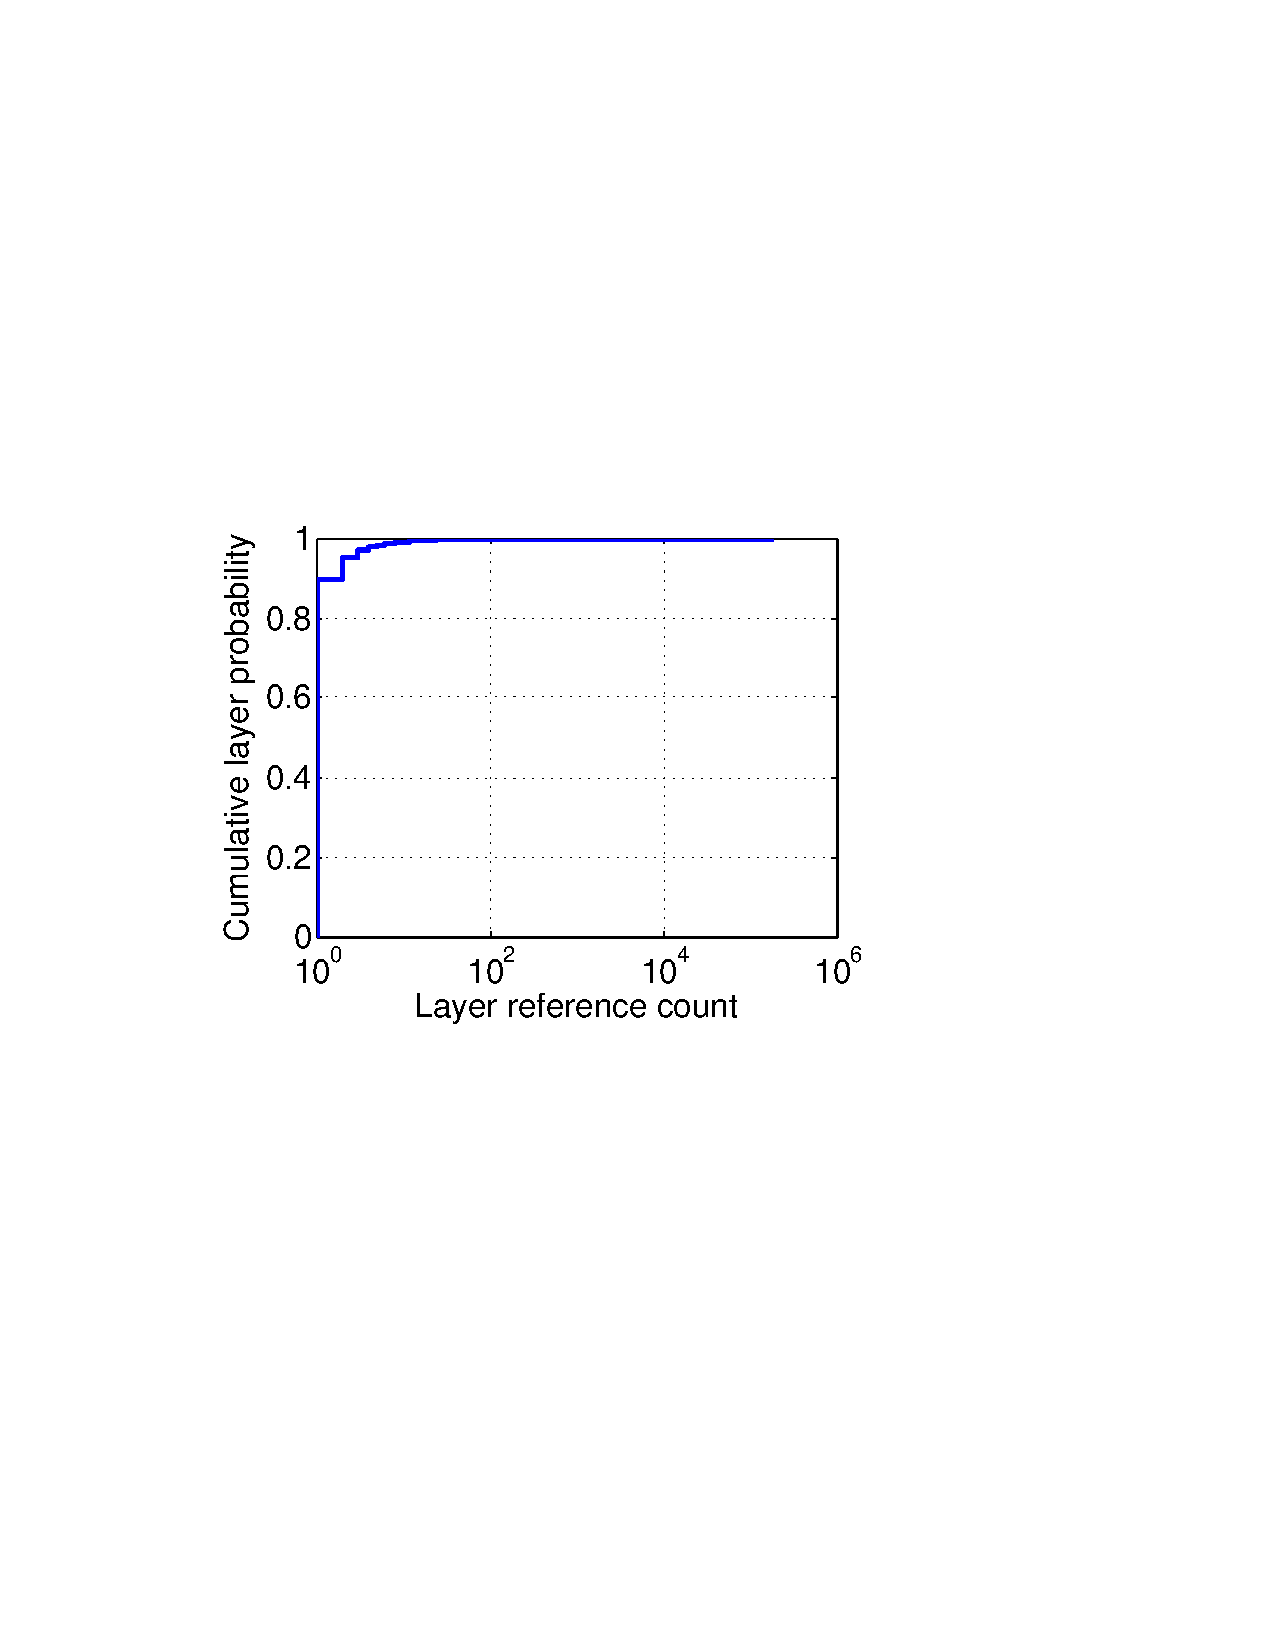
\includegraphics[width=0.21\textwidth]{graphs/shared-cnt-cdf.pdf}
	\caption{CDF of layer reference count.
	}
	\label{fig:ref_count}
\end{figure}


We analyzed all image manifests and count for each layer, how many times it is
referenced by an image.
%
Figure~\ref{fig:ref_count} shows that around 90\% of layers are only reference
by a single image while 95\% are reference by not more than 2 images.
%
Similarly, 99\% of layers are shared among less than 25 images. 
%
Accordingly, we calculated the total storage space consumed before layer-level
content addressability was adopted, which was 84.75 TB.  Thus the redundant
ratio achieved by layer-level content addressability is around 1.8.
%
%Figure~\ref{} shows the absolute values, revealing that almost 1.5 million
%images are only referenced once.  \acomment{Figure is missing} While there is
%again a large spectrum of reference counts, the maximum is 33,428, the vast
%majority of layers is not shared. 
%
This hints that the layer-based approach to improve storage efficiency is
barely utilized and there is room for improvement in how to construct more
sharable layers.
%
\emph{These findings reveal that layer level content addressable store has not
been very successful and most of the layers that exists in Docker Hub are not
shared among images.
	%
	Hence, there is a dire need of a better redundancy management.}

\paragraph{File repeat count}
%\paragraph{Full file duplicates}

\begin{figure} \centering
	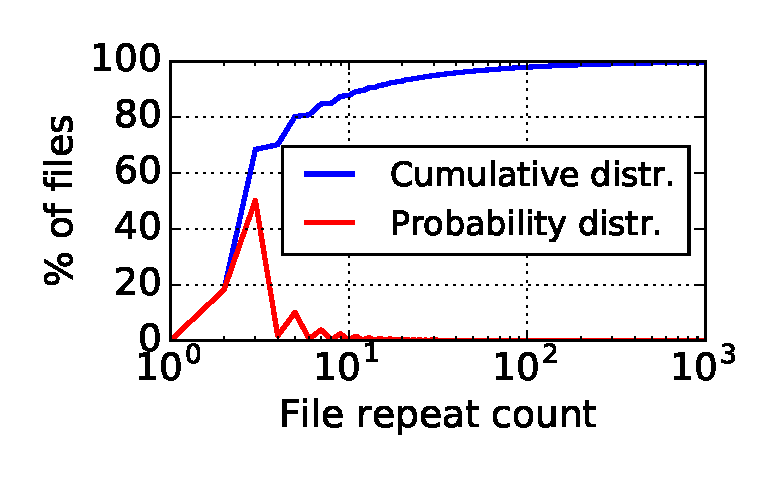
\includegraphics[width=0.45\textwidth]{graphs/File_repeat_count.eps}
	\caption{File repeat count distribution.  } \label{fig:file-repeat-cnt}
\end{figure}

%
Figure~\ref{fig:file-repeat-cnt} shows the cumulative and probability
distribution of file repeat count.  
%
\textit{We see that majority of files have
more than one copies (99.42\%).  
%
Most files have a small repeat count.} For
instance, almost 90\% of files have equal or less than 10 copies. 
%
Around 50\%
of files have 4 copies. 
%
The file that has the maximum repeat count is an empty
file, which means that many users create and store empty files in their images.

\paragraph{Deduplication ratio}
%As discussed in compression ratio analysis, we see that there is redundant
%data in both layers and images.  We conducted simple form of deduplication to
%Interestingly,
Next, we calculate deduplication ratio in terms of file count and capacity for
the complete uncompressed dataset (Table~\ref{tbl:overall-redundant_ratio}).
%the redundant file overhead of the uncompressed dataset 
%
We find that majority of the files have more than one copy (99.42\%), which
take up over 89\% of capacity.  
%
After elimination of file duplicates, the
percentage of such files decrease from 99.42\% to 2.59\%.  
%
Overall, only 3.17\%
(23.92 TB) of files are unique files while 96.83\% of files (143.28 TB) are
redundant copies. 
%
Correspondingly, the deduplication ratio is 96.83\% and
85.69\% in terms of file count and capacity, respectively.
% Table~\ref{tbl:overall-redundant_ratio} summaries the overall redundant file
% overhead in terms of file count and capacity.
%
\textit{Finding 1: Majority of files in Docker registry are duplicates which
occupy most of capacity, indicating that Docker Hub has severe redundancy
problem.}

\begin{table} 
	\centering 
	\scriptsize  
	%\begin{minipage}{.5\linewidth}
	\caption{Redundant ratio in terms of file count and capacity}
	\label{tbl:overall-redundant_ratio} 
	\begin{tabular}{|l|l|l|}%p{0.14\textwidth}
		\hline  
		& File count & Capacity \\ 
		\hline 
		Repeat cnt = 1 & 0.58\% & 10.87\%\\
		\hline 
		Repeat cnt $>$ 1 after dedup. & 2.59\% & 3.44\%\\ 
		\hline 
		Repeat cnt $>$ 1 before dedup.  & 99.42\%  & 89.13\%\\ 
		\hline 
		Unique dataset (Uncompressed) & 3.17\% (167,251,437)  &  14.31\% (23.92 TB) \\ 
		\hline 
		Total dataset (Uncompressed) & 5,278,465,130 & 167.20 TB \\ \hline 	
			%\hline 
	\end{tabular} 
\end{table} 

